Clase: 04/10/2022

\begin{ejemplo}
    Sea la serie $\sum_{n=1}^{\infty} \frac{1}{n^p},p>0\implies a_n=\frac{1}{n^p}$ (positivo y decreciente). Entonces, sea $f(x)=1/x^p (f(n)=1/n^p)$. 
    Sea entonces, 
    Si $p\neq 1$:
    \begin{align}
        \int_1^{\infty}\frac{1}{x^p}dx &= \frac{x^{-p+1}}{-p+1}\Big|_1^{\infty}
    \end{align}
    Si $p>1$ converge, si $p<1$ diverge. 
    
    
    El otro caso, si $p=1$ diverge. 

\end{ejemplo}
\begin{teorema}[Criterio de la integral]
    Suponga que $f$ es una función positiva y decreciente en $[1,\infty)$. Entonces, la serie 
    $\sum_{k=1}^{\infty}a_k$ converge ssi $\int_1^{\infty}f(x)dx$ converge donde $f(k)=a_k,\forall k\in \mathbb{Z}^+$.
    \begin{figure}[H]
        \centering
        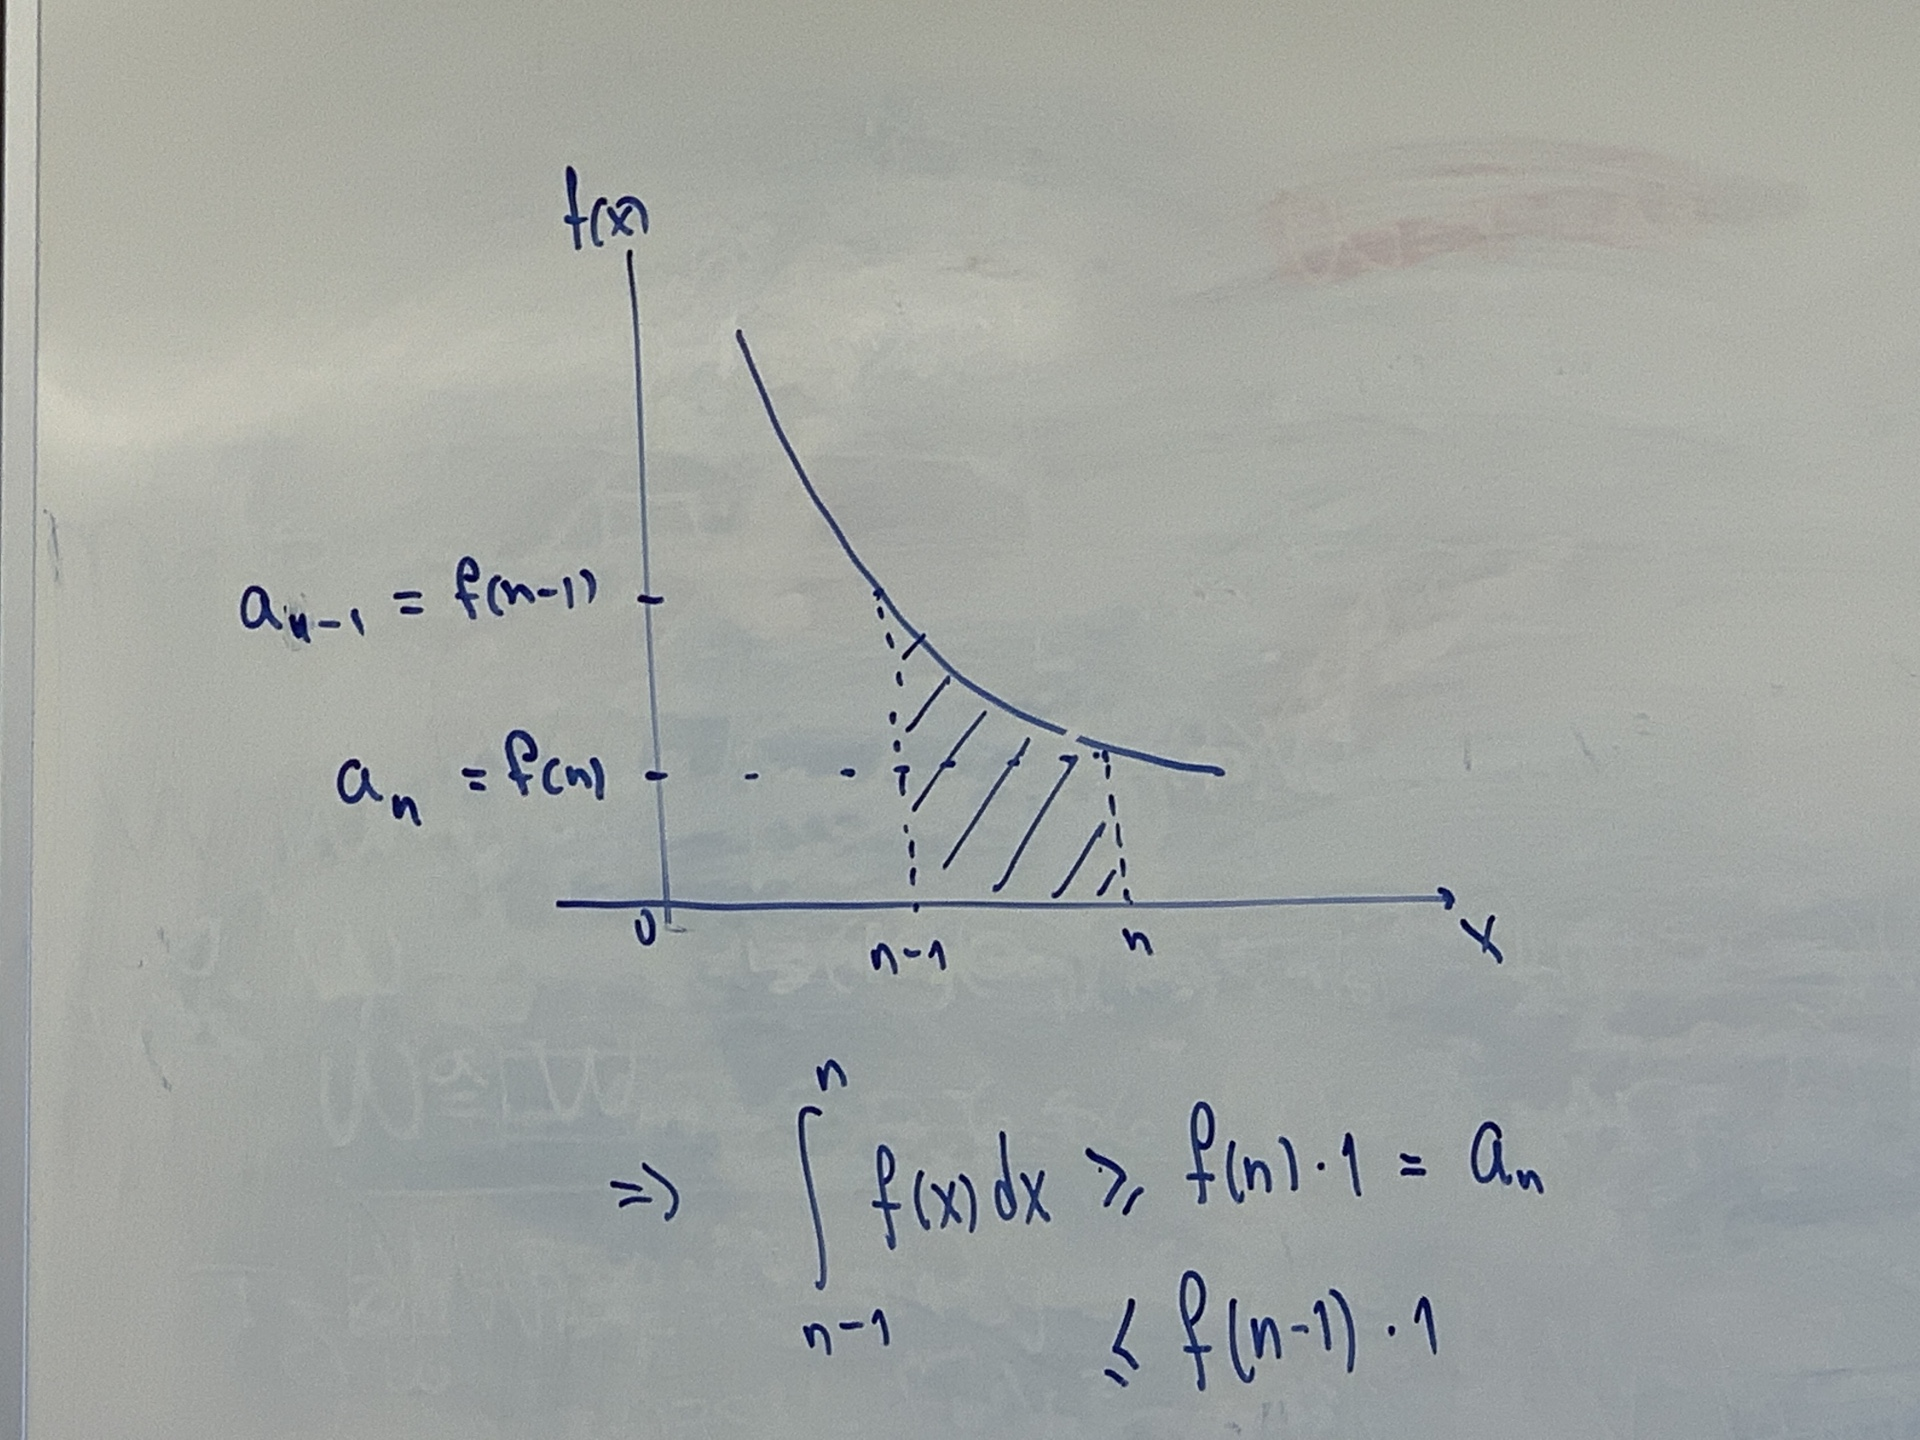
\includegraphics[scale=0.2]{imagenes/18.jpeg}
    \end{figure}
    \begin{dem}
        Se tiene:
        \begin{itemize}
            \item $(\impliedby)$ Suponga que $\int_1^{\infty}f(x)dx$ converge. Se tiene:
            \begin{align*}
                f(2)+f(3)+\cdots + f(k) &\leq \int_1^2 f(x)dx+\int_2^3 f(x)dx +\cdots +\int_{k-1}^k f(x)dx\\
                a_2+a_3+\cdots+a_k&\leq \int_1^k f(x)dx\\
                a_1+\cdots+a_k\leq a_1+\int_1^k f(x)dx
            \end{align*}
            Si $S_k=a_1+\cdots+a_k\implies S_k$ es una sucesión creciente y acotada superiormente $\implies S_k$ converge $\implies \sum_{n=1}^\infty a_k$ converge. 
            \item $(\implies)$ Suponga que $\int_1^{\infty} f(x)dx$ diverge. Nótese que 
            \begin{align*}
                \int_1^2 f(x)dx+\int_2^3 f(x)dx+\cdots +\int_{k}^{k+1}f(x)dx&\leq a_1+a_2+\cdots+a_k
            \end{align*}
            Entonces 
            $$\int_{1}^{k+1}f(x)dx\leq a_1+\cdots+ a_k=S_k$$
            Entonces, la sucesión $S_k$ está acotada inferiormente por una integral divergente, entonces $\sum_{n=1}^\infty a_n$ diverge. 
        \end{itemize}
    \end{dem}
\end{teorema}

\begin{prop}[Criterio de la raíz]
    Sea $\alpha \in \mathbb{R}, 0<\alpha <1$. Si $\sum_{n=1}^\infty a_n$ es t.q., (si para $n\geq N$, se tiene que...) $a_n\geq 0$, 
    $$\sqrt[n]{a_n}\leq\alpha,$$
    entonces $\sum_{n=1}^\infty a_n$ converge. 
    \begin{dem}
        Nótese que, $\forall n\geq N$, se tiene que:
        \begin{align*}
            \sqrt[n]{a_n}&\leq \alpha\\
            a_n&\leq \alpha^n\\
            \sum_{n=N}^{\infty}a_n&\leq \sum_{n=N}^{\infty}\alpha^n\leq \sum_{n=1}^{\infty}\alpha^n,
        \end{align*}
        donde $\sum_{n=1}^\infty \alpha_n$ converge por ser serie geométrica. Entonces, por el criterio de comparación $\sum_{n=N}^{\infty}a_n$ converge $\implies \sum_{n=1}^{\infty} a_n$ converge. 
        \begin{cajita}
            \begin{nota}
                Nótese que si $\forall n\geq N$ se tiene que 
                $$\sqrt[n]{a_n}>1\implies a_n>1\implies \lim_{n\to\infty}a_n\leq 0$$
                Entonces, por criterio de divergencia $\sum_{n=1}^{\infty}a_n$ diverge.
            \end{nota}
        \end{cajita}
    \end{dem}

\end{prop}

\begin{prop}[Criterio de la razón]
    Suponga que para algún $r<1,a_n>0,\forall n\in \mathbb{Z}^+$ se tiene que:
    $$\frac{a_{n+1}}{a_n}\leq r,$$
    entonces $\sum_{n=1}^{\infty}a_n$ converge. 
    \begin{dem}
        Sabemos que 
        \begin{align*}
            a_{n+1}\leq a_n r
        \end{align*}
        Entonces,
        \begin{align*}
            a_{n+2}&\leq a_{n+1}\cdot r\leq a_n r^2\\
            \vdots &\\
            a_{n+k}&\leq a_nr^k
        \end{align*}
        para $n\geq N$, se tiene que 
        $$a_{N+k}\leq a_N r^k$$
        Entonces
        \begin{align*}
            |S_{N+k}-S_N| &= \left| \sum_{n=N}^{N+k}a_n\right|\\
            &= \sum_{k=n}^{N+k}a_n\\
            &\leq a_Nr^k 
        \end{align*}
        Como $r<1\implies S_n$ es de Cauchy. $\implies S_n$ converge $\implies \sum_{n=1}^{\infty}a_n$ converge. 
    \end{dem}
\end{prop}

\begin{teorema}[Convergencia absoluta]
    Si $\sum a_k$ converge absolutamente $\implies \sum a_k$ converge. 
    \begin{dem}
        Si $\sum a_k$ converge absolutamente $\implies |a_k|$ converge $\implies \forall \varepsilon>0\exists N\in \mathbb{Z}^+\ni n\geq N$,
        $$|S_{n+p}-S_n|=\sum_{k=n}^{n+p}|a_k|<\varepsilon,\forall p=1,2,\cdots$$
        Además, sea $S_n'$ la sucesión de sumas parciales de $\sum_{k=1}^\infty a_k$. Entonces, 
        \begin{align*}
            \left| S_{n+p}' -S_n'\right| = \left|\sum_{k=n}^{n+p} a_k\right| \leq \sum_{k=n}^{n+p}|a_k|<\varepsilon
        \end{align*}
        Entonces, $\sum_{k=1}^\infty a_k$ converge.
    \end{dem}
\end{teorema}



\begin{ejemplo}
    Considere la serie $\sum_{n=1}^{\infty}\frac{z^n}{n}$. 
    Considere 
    \begin{align*}
        \left|\frac{z^n}{n}\right| &=\frac{|z|^n}{n}\\
        &\leq |z|^n =r^n
    \end{align*}
    Entonces, tenemos $|z|\leq r$ y 
    $$\sum_{n=1}^{\infty} r^n \leq \sum_{n=0}^{\infty} r^n,$$
    la cual converge para $r<1\implies$ la serie $\sum_{n=1}^{\infty}\frac{z^n}{n}$ converge absolutamente y uniformemente en: 
    $$A_r=\{z\in \mathbb{C}: |z|=r<1\}$$ 
\end{ejemplo}